% !TeX spellcheck = en_US
% !TeX root = ../../build/architecture.tex
% !TeX TXS-program:compile = txs:///xelatex/[--shell-escape]


\renewcommand{\mytitle}{Polygon zkEVM Simplified Processing Flow}
\ifZEROSEC \fi
\ifSEC \section{\mytitle{}}\fi
\ifSUBSEC \subsection{\mytitle{}}\fi
\ifSUBSUBSEC \subsubsection{\mytitle{}}\fi


\begin{frame}{Complete Architecture of the zkEVM}
\begin{figure}
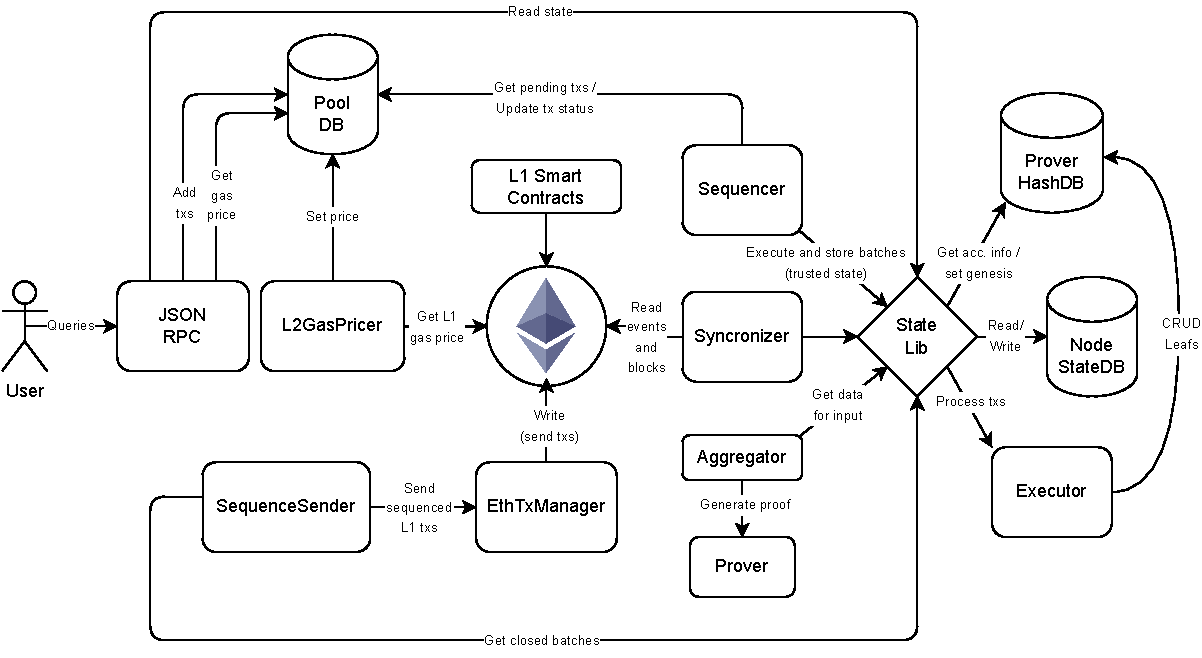
\includegraphics[width=0.8\columnwidth]{\zkevmdir/figures/architecture/zkevm-simplified-flow/architecture-map.drawio}
\end{figure}
\end{frame}




\begin{frame}[t]{Basic zkEVM L2 Processing (Simplified Flow)}
\begin{figure}
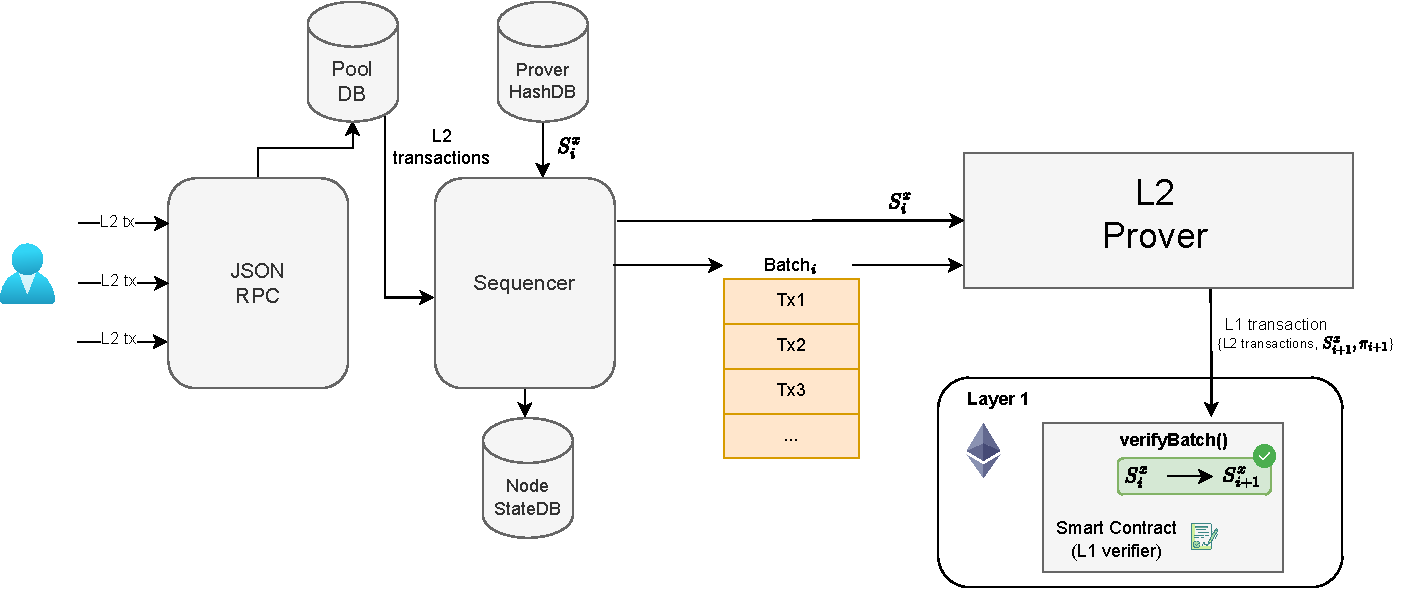
\includegraphics[width=0.95\columnwidth]{\zkevmdir/figures/architecture/zkevm-simplified-flow/zkevm-l2-processing-simplified.drawio}
\end{figure}
\end{frame}




\begin{frame}[allowframebreaks]{Processing an L2 zkEVM Transaction (Simplified Flow)}
\centering
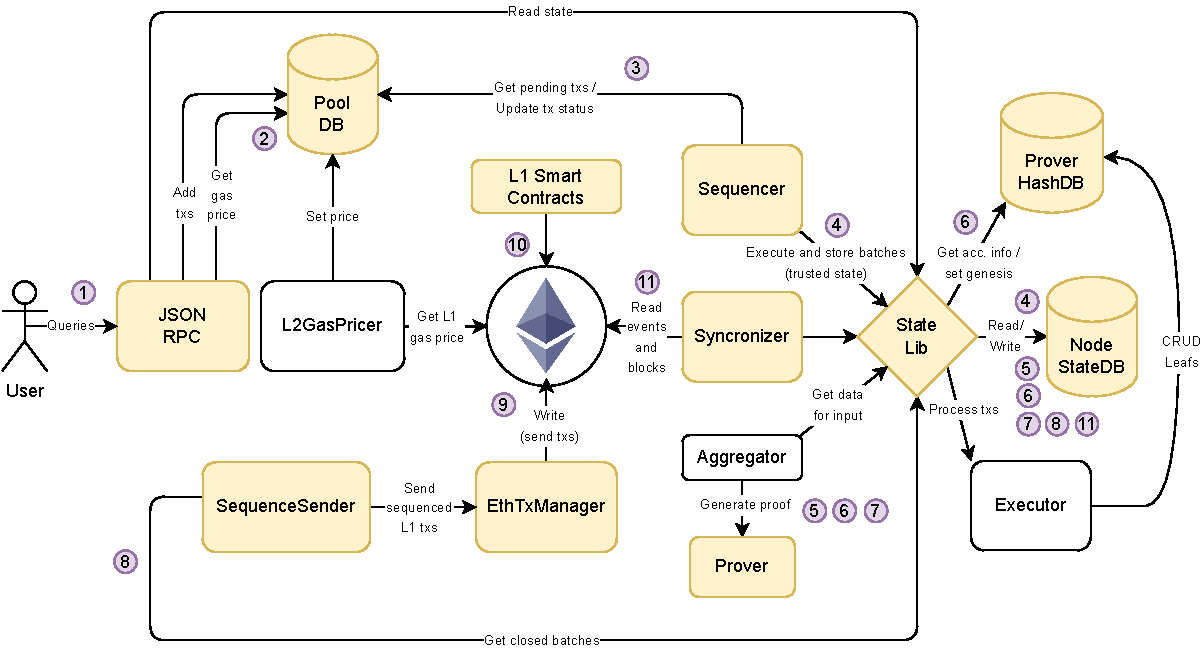
\includegraphics[width=0.8\columnwidth]{\zkevmdir/figures/architecture/zkevm-simplified-flow/architecture-map-simplified-flow.drawio}

\vspace{-0.2cm}
\tiny
\textbf{Remark.} By now, consider that white boxes don't exist. Also take into account that the functionality of some yellow boxes will be re-engineered regarding this simplified flow.

\framebreak
\begin{enumerate}
\small
\item The \textbf{user} creates a standard Ethereum transaction for the L2 (e.g. using the metamask wallet) and, 
sends it to the \textbf{JSON RPC} API of the node, which is an almost standard Ethereum JSON RPC with some extra endpoints.
\item The \textbf{JSON RPC} stores the received L2 transactions in the \textbf{pool} database of pending L2 transactions.
\item The \textbf{sequencer} creates (closes) a batch by selecting L2 transactions from the \textbf{pool} (with some criteria).
\item The \textbf{sequencer} stores the data of the new batch in the node's \textbf{StateDB}.
\item The \textbf{prover} queries the node's \textbf{StateDB} to read the data of the new batches to be proved.
\item The \textbf{prover} also reads the \textbf{HashDB} to obtain the necessary data to proof the current L2 state (root of the L2 state and hashes for Merkle proofs).
\item The \textbf{prover} generates the proof and stores it with its related data in the node's \textbf{StateDB}.

\framebreak
\item The \textbf{sequenceSender} reads the node's \textbf{StateDB} checking for any new proved batches.
\item The \textbf{sequenceSender} decides when it is the best moment to create and send the L1 transaction with the proof to the \textbf{L1 zkEVM smart contract}. The \textbf{sequenceSender} sends the transaction through the \textbf{EthTxManager}. 
The \textbf{EthTxManager} uses an L1 Ethereum node to do so (e.g. \textbf{geth/prysm}) and it makes sure that the transaction is included in a block (managing the L1 gas fees if necessary).
\item The \textbf{L1 zkEVM smart contract} processes the transaction and, if the proof is correctly verified, updates and stores the new L2 state.
\item Finally, the \textbf{synchronizer}, who is monitoring events of the \textbf{L1 zkEVM smart contract} realizes that a new batch is 
consolidated and stores this information in the node's \textbf{StateDB}.
\end{enumerate}
\end{frame}




\begin{frame}[fragile]{Remark About Building the Software}
\begin{itemize}
\item Each component in a box can be instantiated in an isolated executable.
\item The State library is imported by components (is not instantiated).
\item While the JSON RPC is devoted to external communication, 
the component internal communication takes place using two types of interfaces:
  \begin{itemize}
  \item gRPC APIs.
  \item Postgre APIs with the databases.
  \end{itemize}
\item However, many components are built together into a single executable that can 
be configured as desired when started.
\item Finally, remark that the databases can be built as databases in a single Postgre server or
they can be split as desired in multiple PostgreSQL servers.
\end{itemize}
\end{frame}